% ==================================================
% CHAPTER 4: Validating x-ray alignment parameters with cosmic muon data %
% ==================================================

\chapter{Validating x-ray alignment parameters with cosmic muon data}
\label{chap:comparison}
% Edit count: Lia - 0, Brigitte - 0

% --------------------------------------------------
\section{Presentation of theoretical method for comparison}
% --------------------------------------------------

The goal of this work is to validate the alignment parameters extracted from the x-ray data with cosmics data. The crux of the issue is that the x-ray dataset provides absolute local offsets while the cosmics dataset provides relative local offsets. The only solution is to analyze the x-ray data in the same relative coordinate system as cosmics.

The measured beam profile centers provided by the x-ray data were affected by local offsets the same way as cosmics (equation \ref{eqn:local_translation}). Therefore, if a 2-layer track is abstracted from the beam profile center positions on each layer, and the residual calculated on a third layer, that residual should match the cosmics residual. 

Therefore, for each x-ray survey position, the x-ray residual was calculated for all possible tracking combinations (which required an x-ray beam profile on at least three layers). The position of the x-ray residuals are shown as black dots over figure~\ref{fig:res_mean_th2_213} and \ref{fig:res_mean_th2_413}.

The track is "abstracted" because the beam profile center is actually the Gaussian mean of all selected cluster centroids that were recorded during the x-ray data taking period. This was the best analysis method because since the x-rays cause signal in the chamber via the photoeffect, there were not individual "x-ray tracks" to record. In fact the x-ray data was collected separately for each layer. However, since the effect of local offsets on the so-called x-ray residuals would be the same, the difference in algorithm between x-ray and cosmics analysis did not matter. 

% This paragraph is too long and gangly. Reduce it once you're really really sure about the area.
Note that the mean of cosmics residuals around the x-ray points were calculated in bins exactly centered on the nominal x-ray gun position, unlike in FIGURE PREV CHAP OR THIS CHAP??. Several factors went into choosing the area of the region of interest. First, the uncertainty in the cosmics tracks in the x-coordinates for the least geometrically favourable case was just under \SI{40}{\milli\meter}, so the width of the bin in x must be larger than that. But also, the discrete nature of the x-coordinate made it favourable to have bins wider than 2 wire groups, or \SI{72}{\milli\meter} to smooth out the number of entries in each bin. Second, the scale on which local offsets vary by more than \SI{50}{\micro\meter} is \SI{500}{\milli\meter}, assuming a large but possible rotation of \SI{1000}{\micro\radian}. Variations of \SI{50}{\micro\meter} in local offset were deemed significant since the desired position resolution is \SI{100}{\micro\meter}. Therefore, the area had to be significantly lesser than \SI{500}{\milli\meter}. Third, the x-ray gun only covers an area of \SI{20}{\milli\meter} by \SI{20}{\milli\meter}, so ideally only cosmics tracks in that region would be included in the calculation of the mean. However, \SI{20}{\milli\meter} in $x$ is too small and the number of tracks is limited in small bins. Balancing these considerations, \SI{100}{\milli\meter} by \SI{100}{\milli\meter} bins were used. The variation in differences between cosmics residual means for these bins and \SI{40}{\milli\meter} by \SI{20}{\milli\meter} bins is insignificant thanks to the increased statistical uncertainty on the cosmics residual means for the smaller bins.

To  validate the x-ray method, correlation plots were made between the x-ray and cosmics residuals. An example for QL2.P.11 is shown in figure~\ref{fig:correlation}.

\begin{figure}
    \centering
    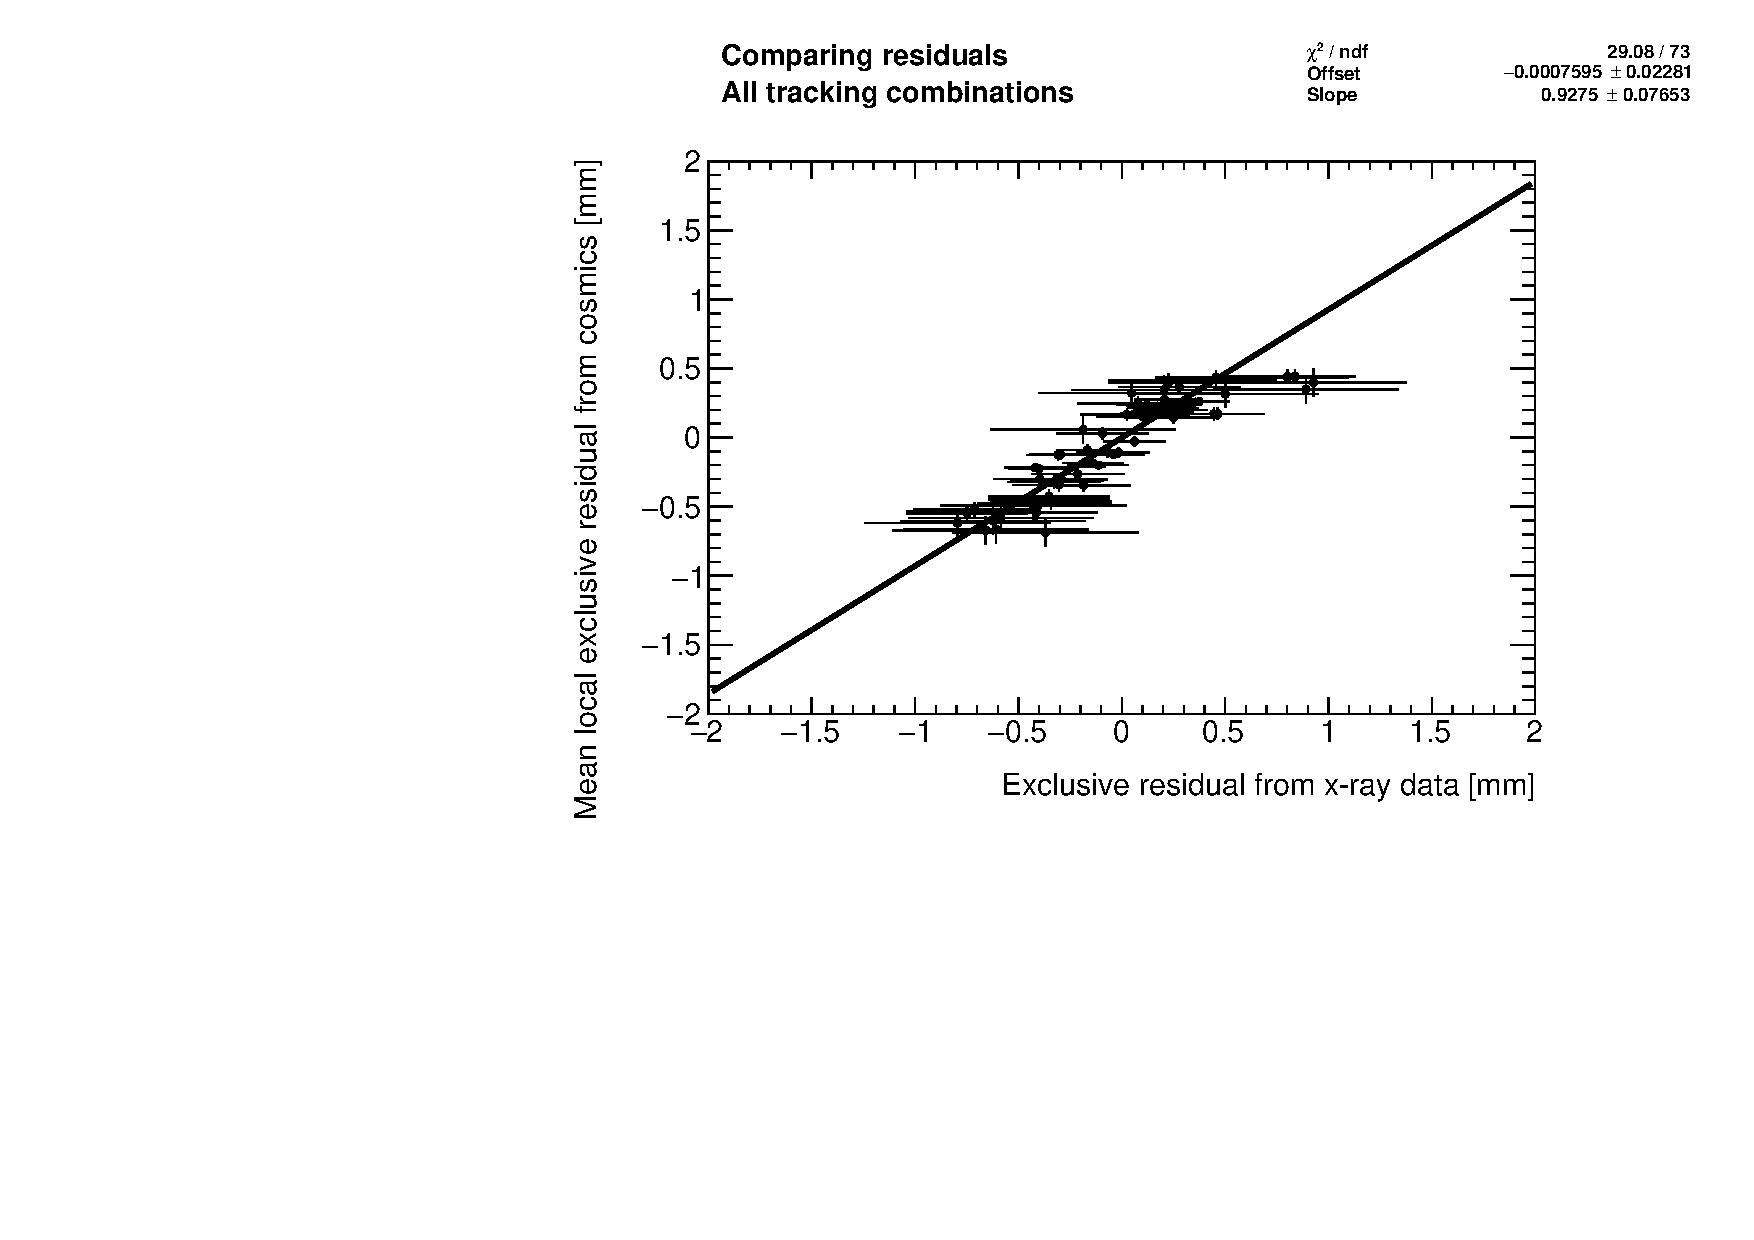
\includegraphics[width = \textwidth]{figures/QL2P11_3100V_2021-08-05_local_mean_cosmics_residual_vs_xray_residual_scatter_all.pdf}
    \caption{Correlation plot between x-ray and cosmics residuals for all tracking combinations for QL2.P.11.}
    \label{fig:correlation}
\end{figure}

First, the fitted slope and offset in figure~\ref{fig:correlation} show that the two datasets largely supported one another for QL2.P.11. However, the magnitude of the uncertainties in the x-ray residuals is large, since it comes from polating the measured x-ray beam centers, which have uncertainty of \SI{120}{\micro\meter} each. The large uncertainty sets a limit on the sensitivity of the analysis, for if the relative offsets of a quadruplet are smaller than the x-ray residual uncertainties, no conclusion on the correlation can be drawn, like for QL2.P.8 (figure~\ref{fig:no_correlation}).

\begin{figure}
    \centering
    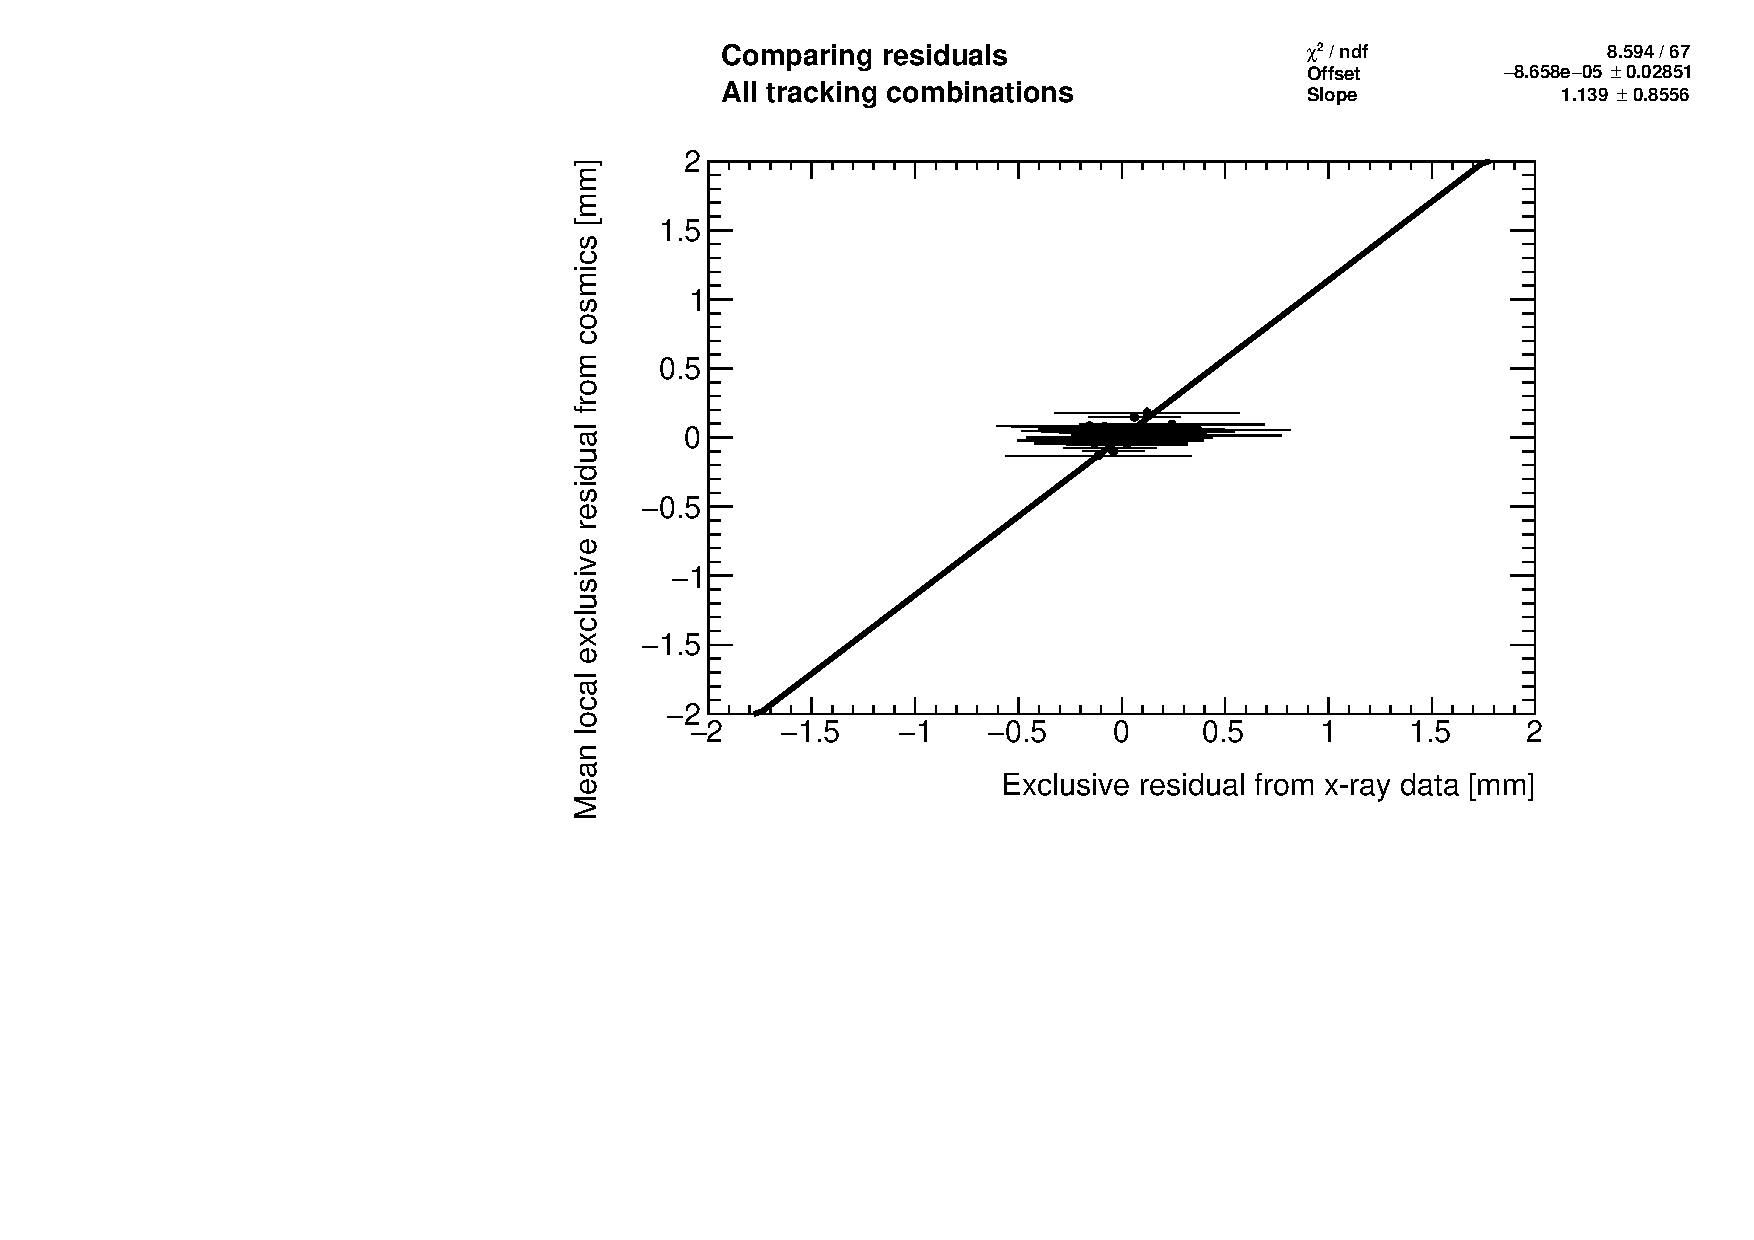
\includegraphics[width = \textwidth]{figures/QL2P08_3100V_2021-07-26_200um_residual_bins_local_mean_cosmics_residual_vs_xray_residual_scatter_all.pdf}
    \caption{Correlation plot between x-ray and cosmics residuals for all tracking combinations for QL2.P.8.}
    \label{fig:no_correlation}
\end{figure}

To say:
- Interps have smaller errors and typically smaller values than extraps
- Uncertainties set the scale on which we are sensitive
- Cosmics has smaller uncertainties => potential to constrain misalignment model with cosmics data.

% Comparing x-ray and cosmics residuals is precisely what was done with the new software package \package{strip_position_analysis}. Several quadruplets of each Canadian geometry were tested using this method, and every possible tracking combination was used to get enough comparison points to check the correlation. 

%TODO : include that x-ray data is collected layer by layer

% --------------------------------------------------
\section{Limitations}
% --------------------------------------------------
An x-ray gun position was only useful if data was recorded on at least 3 layers to be able to calculate a residual. As a result, the number of x-ray residuals for QL2s is around 70 while it is much smaller for QS3Ps.

